% Options for packages loaded elsewhere
\PassOptionsToPackage{unicode}{hyperref}
\PassOptionsToPackage{hyphens}{url}
%
\documentclass[
]{article}
\usepackage{amsmath,amssymb}
\usepackage{lmodern}
\usepackage{iftex}
\ifPDFTeX
  \usepackage[T1]{fontenc}
  \usepackage[utf8]{inputenc}
  \usepackage{textcomp} % provide euro and other symbols
\else % if luatex or xetex
  \usepackage{unicode-math}
  \defaultfontfeatures{Scale=MatchLowercase}
  \defaultfontfeatures[\rmfamily]{Ligatures=TeX,Scale=1}
\fi
% Use upquote if available, for straight quotes in verbatim environments
\IfFileExists{upquote.sty}{\usepackage{upquote}}{}
\IfFileExists{microtype.sty}{% use microtype if available
  \usepackage[]{microtype}
  \UseMicrotypeSet[protrusion]{basicmath} % disable protrusion for tt fonts
}{}
\makeatletter
\@ifundefined{KOMAClassName}{% if non-KOMA class
  \IfFileExists{parskip.sty}{%
    \usepackage{parskip}
  }{% else
    \setlength{\parindent}{0pt}
    \setlength{\parskip}{6pt plus 2pt minus 1pt}}
}{% if KOMA class
  \KOMAoptions{parskip=half}}
\makeatother
\usepackage{xcolor}
\usepackage[margin=0.5in]{geometry}
\usepackage{graphicx}
\makeatletter
\def\maxwidth{\ifdim\Gin@nat@width>\linewidth\linewidth\else\Gin@nat@width\fi}
\def\maxheight{\ifdim\Gin@nat@height>\textheight\textheight\else\Gin@nat@height\fi}
\makeatother
% Scale images if necessary, so that they will not overflow the page
% margins by default, and it is still possible to overwrite the defaults
% using explicit options in \includegraphics[width, height, ...]{}
\setkeys{Gin}{width=\maxwidth,height=\maxheight,keepaspectratio}
% Set default figure placement to htbp
\makeatletter
\def\fps@figure{htbp}
\makeatother
\setlength{\emergencystretch}{3em} % prevent overfull lines
\providecommand{\tightlist}{%
  \setlength{\itemsep}{0pt}\setlength{\parskip}{0pt}}
\setcounter{secnumdepth}{5}
\ifLuaTeX
  \usepackage{selnolig}  % disable illegal ligatures
\fi
\IfFileExists{bookmark.sty}{\usepackage{bookmark}}{\usepackage{hyperref}}
\IfFileExists{xurl.sty}{\usepackage{xurl}}{} % add URL line breaks if available
\urlstyle{same} % disable monospaced font for URLs
\hypersetup{
  pdftitle={Country Summary: Senegal},
  hidelinks,
  pdfcreator={LaTeX via pandoc}}

\title{Country Summary: Senegal}
\author{}
\date{\vspace{-2.5em}}

\begin{document}
\maketitle

{
\setcounter{tocdepth}{2}
\tableofcontents
}
\hypertarget{intro}{%
\section{Intro}\label{intro}}

These estimates are created using a stratified BB8 model with
subnational estimates using a AR1 main temporal effect and a AR1xICAR
spatiotemporal interaction term with area-specific random slopes.

\par

\begin{verbatim}
## Senegal  has  14  Admin 1 areas and  45 Admin 2 areas.
\end{verbatim}

All uncertainty intervals displayed in subsequent figures are 90\%
intervals.

\hypertarget{national-data-summaries-and-results}{%
\section{National Data Summaries and
Results}\label{national-data-summaries-and-results}}

\hypertarget{survey-data}{%
\subsection{Survey data}\label{survey-data}}

\begin{table}[ht]
\centering
\begin{tabular}{cccc}
  \hline
Survey & Urban & Rural & Total \\ 
  \hline
DHS 2015 & 84 & 130 & 214 \\ 
  DHS 2016 & 84 & 130 & 214 \\ 
  DHS 2017 & 186 & 214 & 400 \\ 
  DHS 2018 & 82 & 132 & 214 \\ 
  DHS 2019 & 84 & 130 & 214 \\ 
   \hline
\end{tabular}
\caption{Number of clusters by urban/rural designation by survey for Senegal.} 
\end{table}
\begin{table}[!ht]
\centering
\begin{tabular}{ccc}
   
\multicolumn{3}{l}{DHS 2015}\\ 
\hline
Age & No. Deaths & No. Agemonths \\\hline

0 & 523 & 18258 \\ 
  1-11 & 431 & 189021 \\ 
  12-23 & 232 & 192747 \\ 
  24-35 & 146 & 180907 \\ 
  36-47 & 106 & 168989 \\ 
  48-59 & 64 & 157496 \\ 
   \hline\\ 
\multicolumn{3}{l}{DHS 2016}\\ 
\hline
Age & No. Deaths & No. Agemonths \\\hline
0 & 485 & 18513 \\ 
  1-11 & 363 & 192626 \\ 
  12-23 & 196 & 197344 \\ 
  24-35 & 162 & 185967 \\ 
  36-47 & 115 & 173441 \\ 
  48-59 & 63 & 161487 \\ 
   \hline\\ 
\multicolumn{3}{l}{DHS 2017}\\ 
\hline
Age & No. Deaths & No. Agemonths \\\hline
0 & 1078 & 36086 \\ 
  1-11 & 718 & 374844 \\ 
  12-23 & 375 & 385329 \\ 
  24-35 & 226 & 363821 \\ 
  36-47 & 177 & 342816 \\ 
  48-59 & 108 & 320512 \\ 
   \hline\\ 
\multicolumn{3}{l}{DHS 2018}\\ 
\hline
Age & No. Deaths & No. Agemonths \\\hline
0 & 547 & 20753 \\ 
  1-11 & 385 & 216071 \\ 
  12-23 & 204 & 221539 \\ 
  24-35 & 129 & 209183 \\ 
  36-47 & 106 & 196784 \\ 
  48-59 & 60 & 183603 \\ 
   \hline\\ 
\multicolumn{3}{l}{DHS 2019}\\ 
\hline
Age & No. Deaths & No. Agemonths \\\hline
0 & 509 & 19257 \\ 
  1-11 & 362 & 199496 \\ 
  12-23 & 151 & 204486 \\ 
  24-35 & 109 & 192117 \\ 
  36-47 & 76 & 180258 \\ 
  48-59 & 44 & 168796 \\ 
   \hline
\multicolumn{3}{l}{}\\
\end{tabular}
\caption{Numbers of agemonths and deaths by age group for each survey used in analysis for Senegal.} 
\end{table}

\begin{table}[ht]
\centering
\begin{tabular}{l|cc}
  \hline
Age & urban & rural \\ 
  \hline
0 & (21.7,26) & (25.2,29.2) \\ 
  1-11 & (1.2,1.5) & (1.7,2) \\ 
  12-23 & (0.4,0.5) & (0.9,1) \\ 
  24-35 & (0.3,0.4) & (0.6,0.8) \\ 
  36-47 & (0.2,0.4) & (0.5,0.6) \\ 
  48-59 & (0.2,0.3) & (0.3,0.4) \\ 
   \hline
\end{tabular}
\caption{The 95\% credible intervals for monthly hazards in terms of 1000 children by age band for the Admin-1, benchmarked stratified model for Senegal.} 
\end{table}

\clearpage

\hypertarget{figures}{%
\subsection{Figures}\label{figures}}

\begin{figure}
 \centering
\includegraphics[width=5in]{U:/UN-Subnational-Estimates/Results/Senegal/Figures/Trends/U5MR/Senegal_URodds_natl_ar1_strat_u5.pdf}
\caption{Urban rural odds ratio from stratified national model.}
\end{figure}
\clearpage

\begin{figure}
 \centering
\includegraphics[width=7.5in]{U:/UN-Subnational-Estimates/Results/Senegal/Figures/Summary/NMR/Senegal_natl_strat_ar1_nmr_Spaghetti.pdf}
\caption{NMR results from the national BB8 model.}
\end{figure}
\begin{figure}
 \centering
\includegraphics[width=7.5in]{U:/UN-Subnational-Estimates/Results/Senegal/Figures/Summary/U5MR/Senegal_natl_strat_ar1_u5_Spaghetti.pdf}
\caption{U5MR results from the national BB8 model.}
\end{figure}
\clearpage

\clearpage

\hypertarget{subnational-results}{%
\section{Subnational Results}\label{subnational-results}}

\begin{figure}[!h]
 \centering
\includegraphics[width=3.5in]{U:/UN-Subnational-Estimates/Results/Senegal/Figures/ShapeCheck/Senegal_adm1_neighb.pdf}
\includegraphics[width=3.5in]{U:/UN-Subnational-Estimates/Results/Senegal/Figures/ShapeCheck/Senegal_adm2_neighb.pdf}
\caption{Top: The neighborhood structure of Admin 1 areas. Bottom: The neighborhood structure of Admin 2 areas.}
\end{figure}

\hypertarget{admin-1-figures}{%
\subsection{Admin 1 Figures}\label{admin-1-figures}}

\begin{figure}[!h]
 \centering
\includegraphics[width=3.5in]{U:/UN-Subnational-Estimates/Results/Senegal/Figures/Summary/NMR/Senegal_adm1_ar1_strat_nmr_bench_medianmap_20002021.pdf}
\includegraphics[width=3.5in]{U:/UN-Subnational-Estimates/Results/Senegal/Figures/Summary/U5MR/Senegal_adm1_ar1_strat_u5_bench_medianmap_20002021.pdf}
\caption{NMR (left) and U5MR (right) results in 2000, 2010, 2015, and 2021 from the Admin-1 BB8 model.}
\end{figure}
\clearpage

\begin{figure}[!h]
 \centering
\includegraphics[width=7.5in]{U:/UN-Subnational-Estimates/Results/Senegal/Figures/Summary/NMR/Senegal_Admin1_nmr_SpaghettiAll_ar1_strat_bench_1.pdf}
\end{figure}
\clearpage

\begin{figure}[!h]
 \centering
\includegraphics[width=7.5in]{U:/UN-Subnational-Estimates/Results/Senegal/Figures/Summary/U5MR/Senegal_Admin1_u5_SpaghettiAll_ar1_strat_bench_1.pdf}
\end{figure}

\clearpage

\hypertarget{admin-2-figures}{%
\subsection{Admin 2 Figures}\label{admin-2-figures}}

\begin{figure}[!h]
 \centering
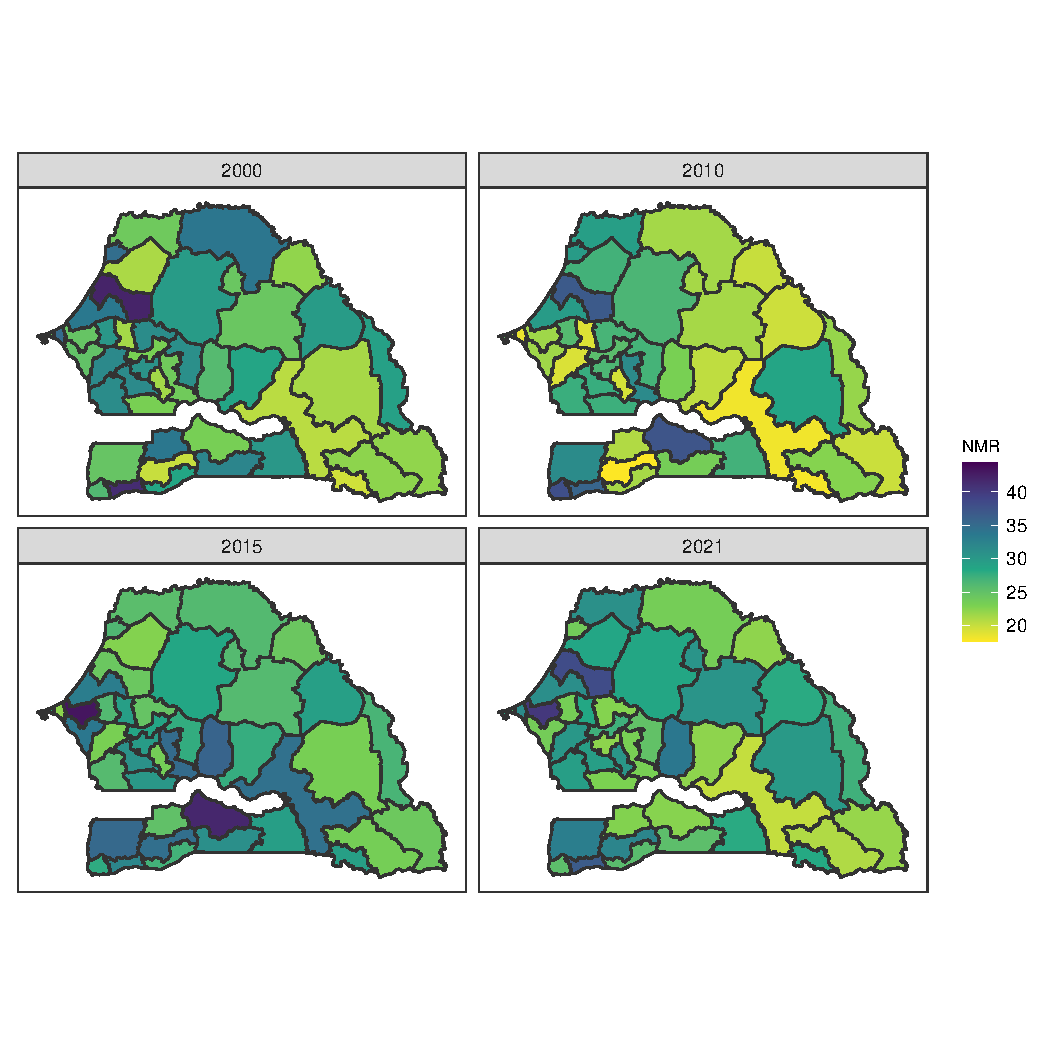
\includegraphics[width=3.5in]{U:/UN-Subnational-Estimates/Results/Senegal/Figures/Summary/NMR/Senegal_adm2_ar1_strat_nmr_bench_medianmap_20002021.pdf}
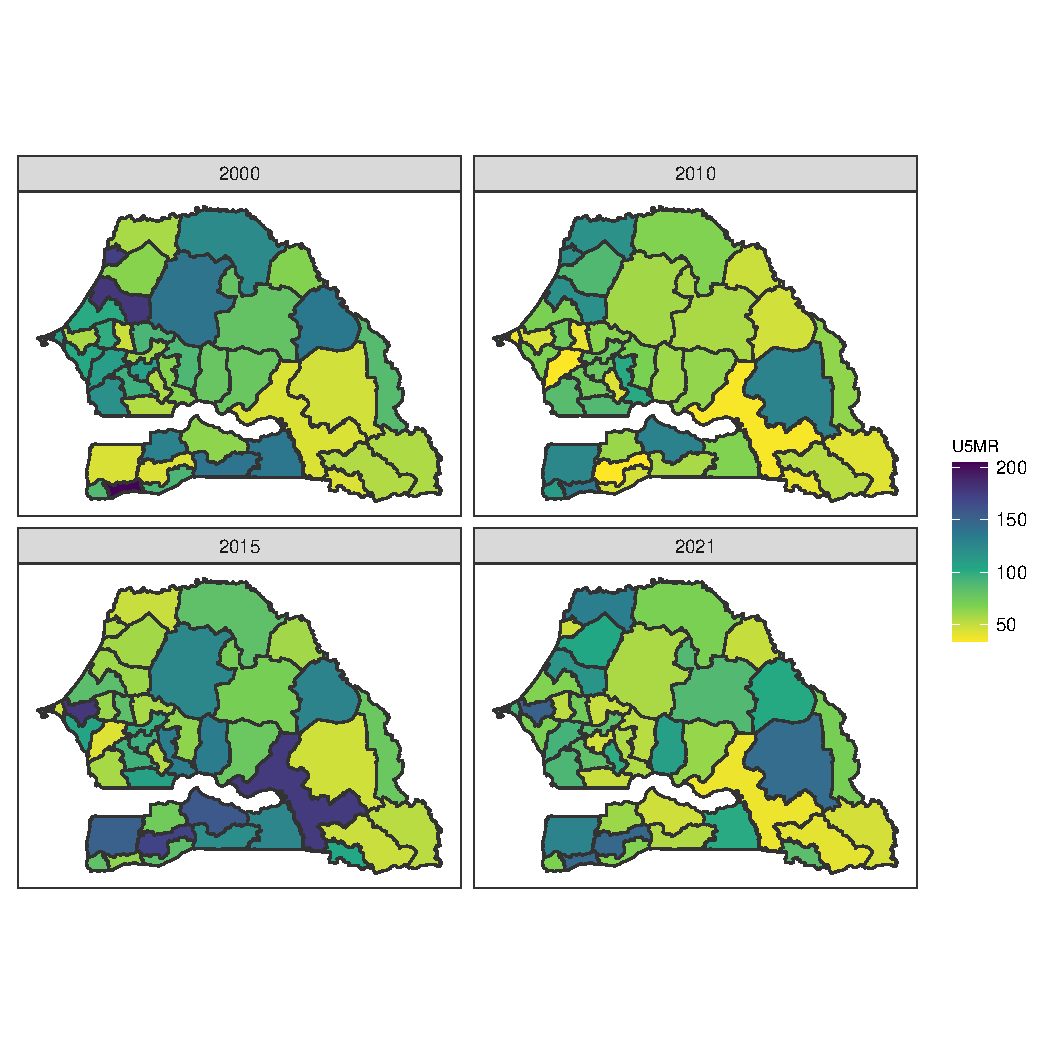
\includegraphics[width=3.5in]{U:/UN-Subnational-Estimates/Results/Senegal/Figures/Summary/U5MR/Senegal_adm2_ar1_strat_u5_bench_medianmap_20002021.pdf}
\caption{NMR (left) and U5MR (right) results in 2000, 2010, 2015, and 2021 from the Admin-2 BB8 model.}
\end{figure}
\clearpage

\begin{figure}[!h]
 \centering
\includegraphics[width=7.5in]{U:/UN-Subnational-Estimates/Results/Senegal/Figures/Summary/NMR/Senegal_Admin2_nmr_SpaghettiAll_ar1_strat_bench_1.pdf}
\end{figure}
\begin{figure}[!h]
 \centering
\includegraphics[width=7.5in]{U:/UN-Subnational-Estimates/Results/Senegal/Figures/Summary/NMR/Senegal_Admin2_nmr_SpaghettiAll_ar1_strat_bench_2.pdf}
\end{figure}
\begin{figure}[!h]
 \centering
\includegraphics[width=7.5in]{U:/UN-Subnational-Estimates/Results/Senegal/Figures/Summary/NMR/Senegal_Admin2_nmr_SpaghettiAll_ar1_strat_bench_3.pdf}
\end{figure}
\clearpage
\begin{figure}[!h]
 \centering
\includegraphics[width=7.5in]{U:/UN-Subnational-Estimates/Results/Senegal/Figures/Summary/U5MR/Senegal_Admin2_u5_SpaghettiAll_ar1_strat_bench_1.pdf}
\end{figure}
\begin{figure}[!h]
 \centering
\includegraphics[width=7.5in]{U:/UN-Subnational-Estimates/Results/Senegal/Figures/Summary/U5MR/Senegal_Admin2_u5_SpaghettiAll_ar1_strat_bench_2.pdf}
\end{figure}
\begin{figure}[!h]
 \centering
\includegraphics[width=7.5in]{U:/UN-Subnational-Estimates/Results/Senegal/Figures/Summary/U5MR/Senegal_Admin2_u5_SpaghettiAll_ar1_strat_bench_3.pdf}
\end{figure}

\end{document}
